\documentclass[10pt, landscape]{article}
\usepackage[scaled=0.92]{helvet}
\usepackage{calc}
\usepackage{graphicx}
\usepackage{multicol}
\usepackage{ifthen}
\usepackage[a4paper,margin=3mm,landscape]{geometry}
\usepackage{amsmath,amsthm,amsfonts,amssymb}
\usepackage{color,graphicx,overpic}
\usepackage{hyperref}
\usepackage{newtxtext} 
\usepackage{enumitem}
\usepackage{graphicx}
\usepackage[table]{xcolor}
\usepackage{mathtools}
\usepackage[document]{ragged2e}
\usepackage{listings}
\setlist{nosep}
\usepackage{subfig}


% for including images
\graphicspath{ {./images/} }


\pdfinfo{
  /Title (CS3223.pdf)
  /Creator (TeX)
  /Producer (pdfTeX 1.40.0)
  /Author (Pei Cheng Yi)
  /Subject (CS3223)
  /Keywords (CS3223, nus,cheatsheet,pdf)}

% Turn off header and footer
\pagestyle{empty}

\newenvironment{tightcenter}{%
  \setlength\topsep{0pt}
  \setlength\parskip{0pt}
  \begin{center}
}{%
  \end{center}
}

% redefine section commands to use less space
\makeatletter
\renewcommand{\section}{\@startsection{section}{1}{0mm}%
                                {-1ex plus -.5ex minus -.2ex}%
                                {0.5ex plus .2ex}%x
                                {\normalfont\large\bfseries}}
\renewcommand{\subsection}{\@startsection{subsection}{2}{0mm}%
                                {-1explus -.5ex minus -.2ex}%
                                {0.5ex plus .2ex}%
                                {\normalfont\normalsize\bfseries}}
\renewcommand{\subsubsection}{\@startsection{subsubsection}{3}{0mm}%
                                {-1ex plus -.5ex minus -.2ex}%
                                {1ex plus .2ex}%
                                {\normalfont\small\bfseries}}%
\renewcommand{\familydefault}{\sfdefault}
\renewcommand\rmdefault{\sfdefault}
%  makes nested numbering (e.g. 1.1.1, 1.1.2, etc)
\renewcommand{\labelenumii}{\theenumii}
\renewcommand{\theenumii}{\theenumi.\arabic{enumii}.}
\renewcommand\labelitemii{•}
\renewcommand\labelitemiii{•}
%  convenient absolute value symbol
\newcommand{\abs}[1]{\vert #1 \vert}
%  convenient floor and ceiling
\newcommand{\floor}[1]{\lfloor #1 \rfloor}
\newcommand{\ceil}[1]{\lceil #1 \rceil}
%  convenient modulo
\newcommand{\Mod}[1]{\ \mathrm{mod}\ #1}
%  for logical not operator, iff symbol, convenient "if/then"
\renewcommand{\lnot}{\mathord{\sim}}
\let\then\Rightarrow
\let\Then\Rightarrow
%  vectors
\newcommand{\vv}[1]{\boldsymbol{#1}}
\newcommand{\VV}[1]{\overrightarrow{#1}}
%  column vector
\newcommand{\cvv}[1]{\left(\begin{smallmatrix}#1\end{smallmatrix}\right)}
\newcommand{\code}[1]{\textcolor{myblue}{\texttt{#1}}}
\newcommand\bggreen{\cellcolor{green!10}}

\makeatother
\definecolor{myblue}{cmyk}{1,.72,0,.38}
\everymath\expandafter{\the\everymath \color{myblue}}
% Define BibTeX command
\def\BibTeX{{\rm B\kern-.05em{\sc i\kern-.025em b}\kern-.08em
    T\kern-.1667em\lower.7ex\hbox{E}\kern-.125emX}}

% Don't print section numbers
\setcounter{secnumdepth}{0}

\setlength{\parindent}{0pt}
\setlength{\parskip}{0pt plus 0.5ex}
%% this changes all items (enumerate and itemize)
\setlength{\leftmargini}{0.5cm}
\setlength{\leftmarginii}{0.4cm}
\setlength{\leftmarginiii}{0.5cm}
\setlist[enumerate,1]{leftmargin=2mm,labelindent=1mm,labelsep=1mm}
\setlist[itemize,1]{leftmargin=2mm,labelindent=1mm,labelsep=1mm}
\setlist[itemize,2]{leftmargin=3mm,labelindent=1mm,labelsep=1mm}
\setlist[itemize,3]{leftmargin=3mm,labelindent=1mm,labelsep=1mm}

%My Environments
\newtheorem{example}[section]{Example}
% -----------------------------------------------------------------------

\begin{document}
\raggedright
\footnotesize
\begin{multicols}{4}


% multicol parameters
% These lengths are set only within the two main columns
\setlength{\columnseprule}{0.25pt}
\setlength{\premulticols}{1pt}
\setlength{\postmulticols}{1pt}
\setlength{\multicolsep}{1pt}
\setlength{\columnsep}{2pt}

\begin{center}
    \fbox{%
        \parbox{0.8\linewidth}{\centering \textcolor{black}{
            {\Large\textbf{CS3223}}
            \\ \normalsize{AY22/23 Sem 2}}
            \\ {\footnotesize \textcolor{myblue}{github.com/SeekSaveServe}}
        }%
    }
\end{center}

\section{L1 - Data Storage}
\subsection{Magnetic Disks}

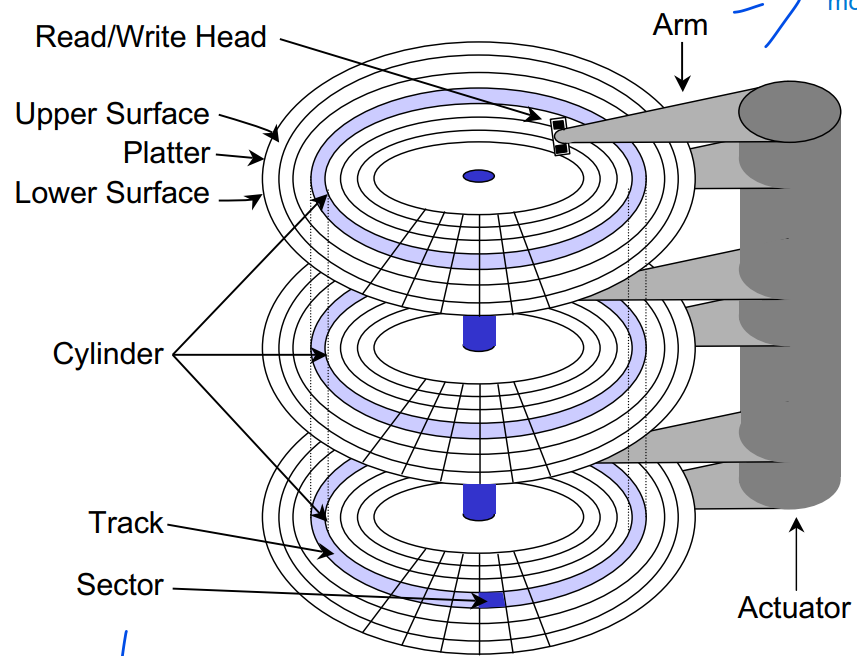
\includegraphics[width=3.5cm, height =2cm]{magnetic_disk.png}

\begin{itemize}
    \item \textbf{Disk Access Time} Seek time + Rotational Latency + Transfer time
    \item \textbf{Response time} Queueing delay + Disk access time
    \item \textbf{Rotational Delay} $\frac{1}{2} \frac{60s}{RPM}$ 
    \item \textbf{Transfer Time} sectors on the same track * $\tfrac{Time Per Revolution}{Sectors Per Track}$
\end{itemize}

\subsection{Buffer Manager}
\begin{itemize}
  \item \textbf{Buffer pool} Main memory allocated for DBMS
  \item \textbf{pin count} is incremented upon pinning
  \item \textbf{dirty bit} is updated when the page is unpinned (if modified)
  \item \textbf Replacement is only possbile if pin count == 0 
\end{itemize}

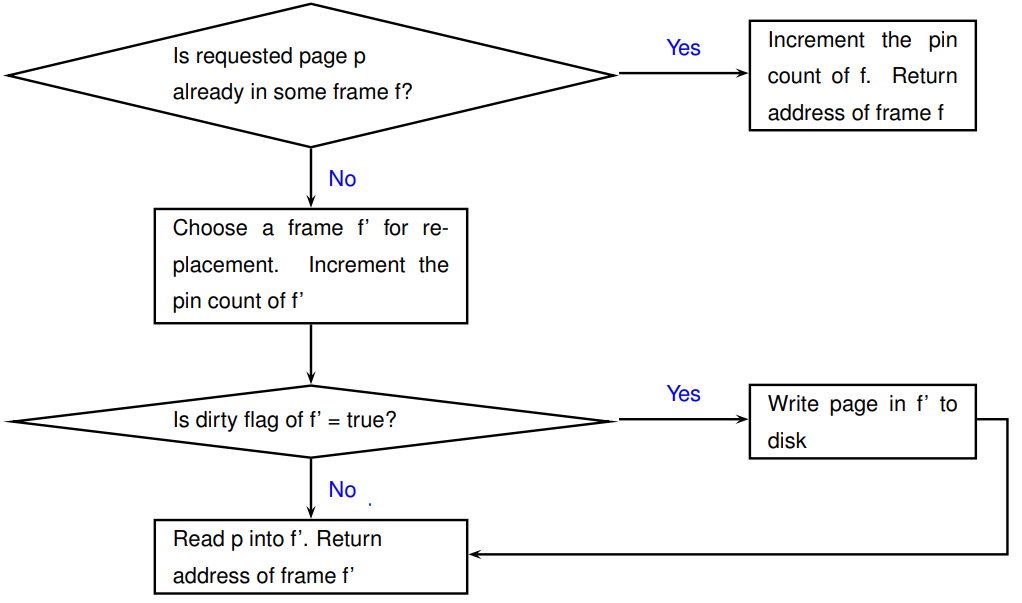
\includegraphics[width=5cm, height =3.5cm]{buff_manager_handle_request.png}

\subsection{Replacement Policies}
\textbf{LRU Policy}
\begin{itemize}
  \item Maintains a queue of pointers to frames with pin count = 0
\end{itemize}


\textbf{Clock Replacement Policy}
\includegraphics*[width=5cm, height=3.5cm]{clock.png}
\begin{itemize}
  \item Simplifies LRU with a second chance round robin system
  \item Each frame has a \textcolor{red}{reference bit} that is turned on when pin count reaches 0
  \item Repalces a page when referenced bit if off and pin count is 0
\end{itemize}

\subsection{File Organisation}
\includegraphics*[width=7cm, height=4cm]{heap_file.png}

\textbf{Page Formats: Fixed Length Records}
\begin{itemize}
  \item \textbf{Packed Organisation} Store records in contiguous slots
  \item \textbf{Unpacked Organisation} Uses a bit array to maintain free slots
\end{itemize}

\includegraphics*[width=7cm, height=4cm]{page_org.png}


\textbf{Page Formats: Slotted Page (variable length record)}
\begin{itemize}
  \item Store records in slots of \textsl{(record offset, record length)}
  \item Record Offset: Offset of the record from the start of the page
\end{itemize}

\includegraphics*[width=7cm, height=4cm]{slot_page.png}

\textbf{Record Formats}
\begin{itemize}
  \item 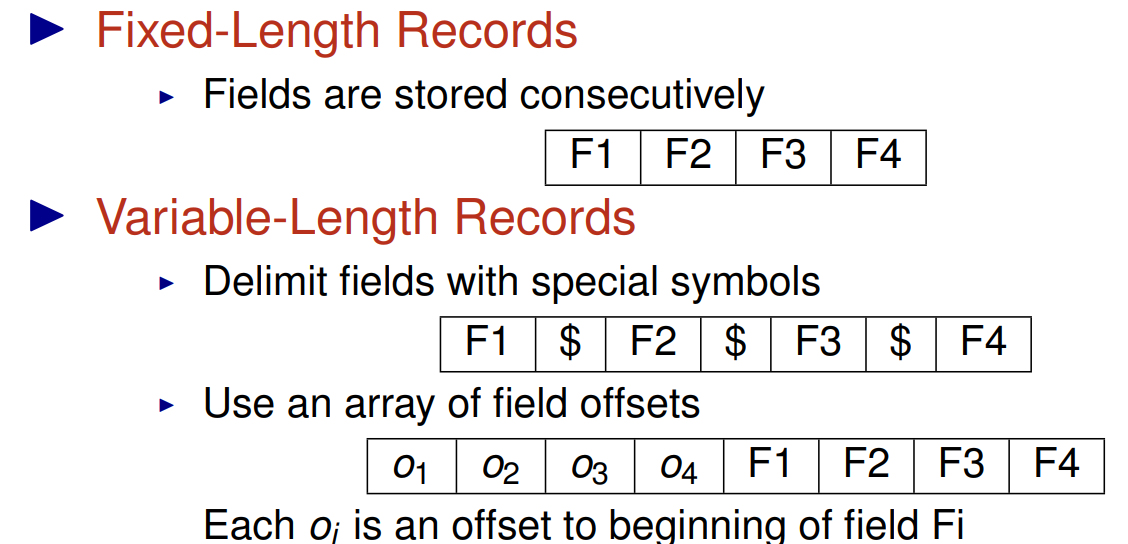
\includegraphics[width=3.5cm, height=2cm]{var_record.png}
\end{itemize}


\section{L2 And L3 - Indexing}
\begin{itemize}
  \item A search key is a sequence of k attributes. If k > 1, composite key
  \item A search key is an unique index if it is a candidate key
  \item An index is stored as a file
\end{itemize}

\textbf{Format of data entries}
\begin{itemize}
  \item Format 1: k* is an actual data record with search value k
  \item Format 2: k* is the form (k, rid)
  \item Format 3: k* is the form (k, rid-list*)
  \item Note: Different formats affects the number of data entries stored in a page
\end{itemize}

\textbf{Clustered Vs Unclustered}
\begin{itemize}
  \item \textcolor{red}{Clustered}: Order of data entries is the same as the oreder of data records. Can only be built on ordered field (e.g. primary key)
  \item \textcolor{green}{Unclustered}: Order of data entries does not correspond to the order of data records
  \item The implication is that we can read an entire clustered page with 1 I/O
  \item  B+ Tree: Format 1 is clustered, Format 2 and 3 can be clustered if data records are sorted on the search key
  \item Hash: Only format 1 is clustered since hashing do not store data entries in search key order
\end{itemize}

\textbf{Tree Based Index - B+ Tree}
\begin{itemize}
  \item Leaf nodes are doubly linked and store Data Entries
  \item Internal nodes sotre index entries (p0, k, p1 ... pk, k, pk+1)
  \item Internal nodes contains m entries,  m $\in$ [d, 2d] $\rightarrow$ space utilisation $\geq$ 50\%
  \item Root contains m entries, m $\in$ [1, 2d]
\end{itemize}

\textbf{B+ Tree - Split Overflow Nodes}
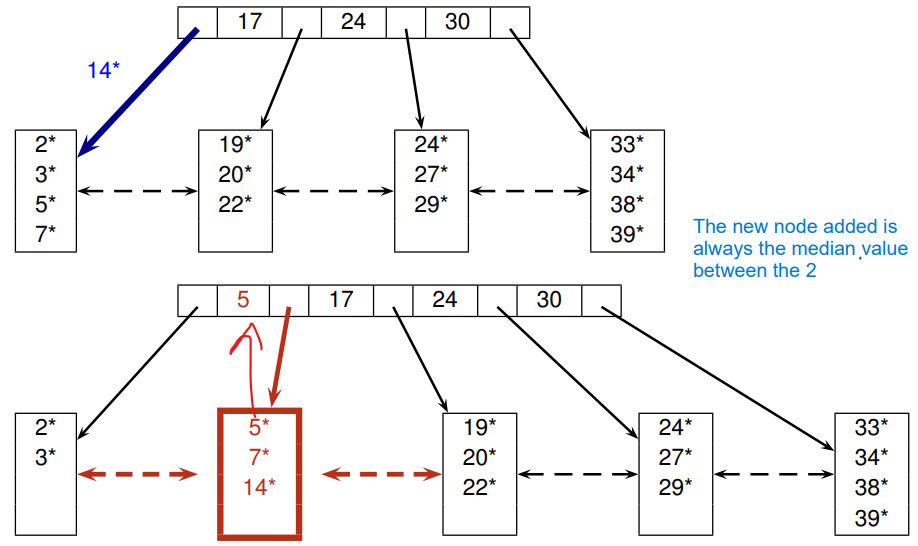
\includegraphics[width=7cm, height=4cm]{split_overflow_node.png}
\begin{itemize}
  \item Distribute d+1 entries to the new leaf node
  \item Create new entry index using smallest key in the new node (middle key)
  \item Insert new entry into parent node of overflowed node
\end{itemize}

\textbf{B+ Tree - Overflow Propagation}
\newline
5 is pushed up
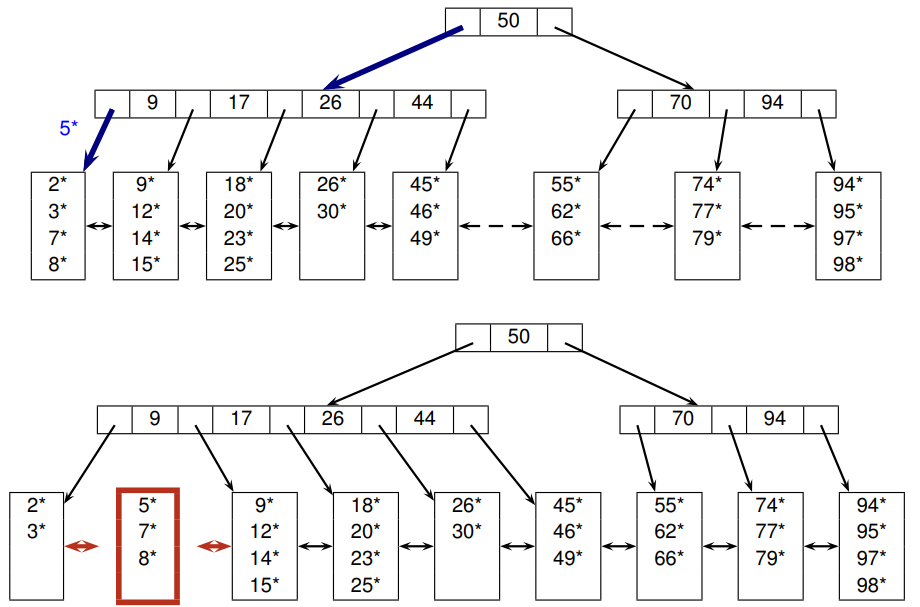
\includegraphics[width=7cm, height=4cm]{overflow_progpagation1.png}
17 is pushed up
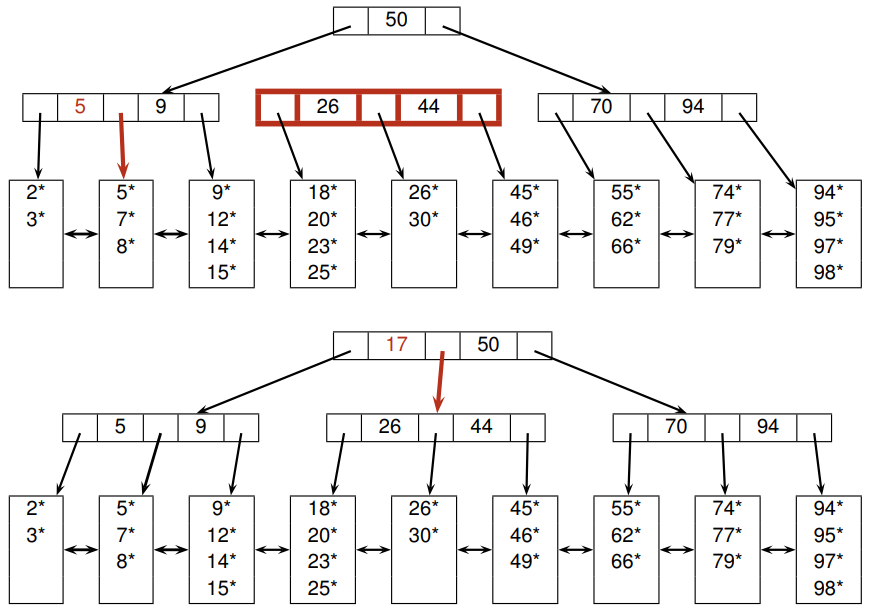
\includegraphics[width=7cm, height=4cm]{overflow_progpagation2.png}

\begin{itemize}
  \item Excess middle node is pushed updated to parent node
\end{itemize}

\textbf{B+ Tree - Redistribution of data entries}
\begin{itemize}
  \item Two nodes are siblings if they have the same parent node
\end{itemize}
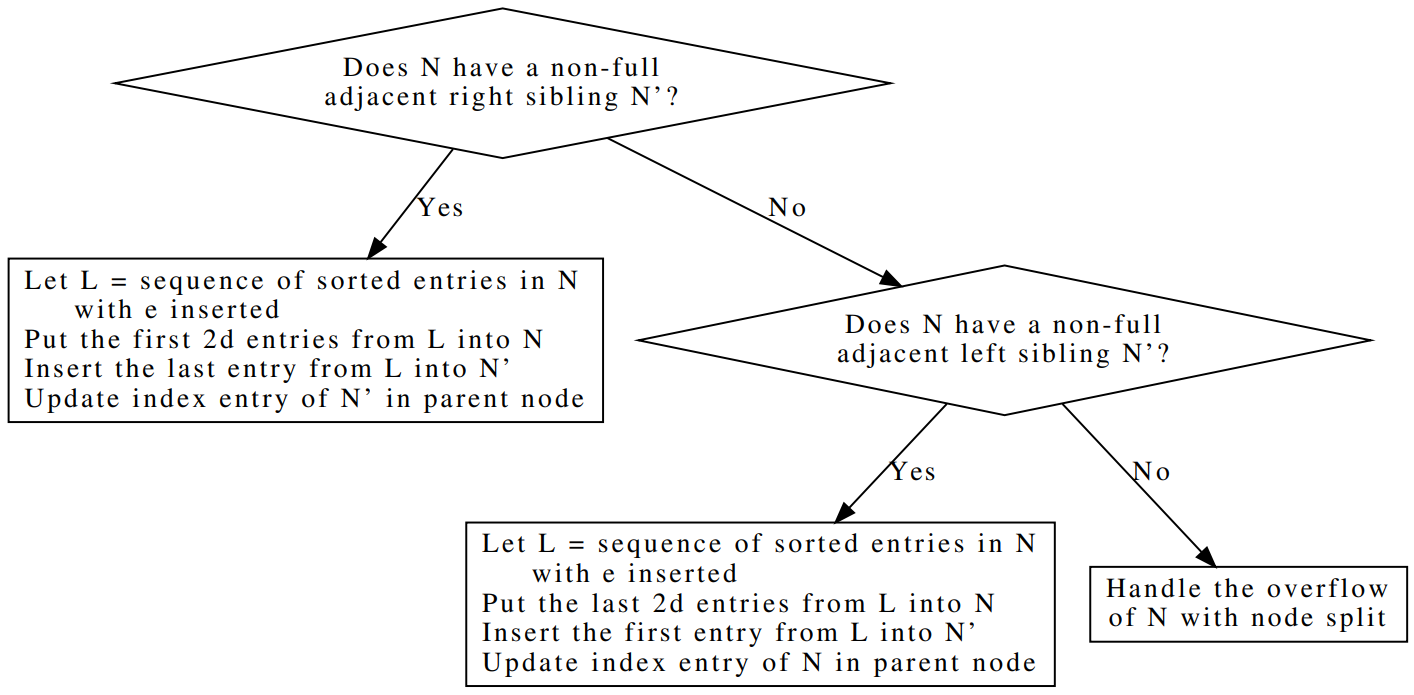
\includegraphics[width=7cm, height=4cm]{overflow_redistribution.png}

\textbf{B+ Tree - Underflow}
\begin{itemize}
  \item Underflow occurs when a node has less than d entries
  \item Underflow is resolved by redistributing entries between siblings
  \item An underflow node is merged if each of its adjacent siblings have exactly d entries
\end{itemize}

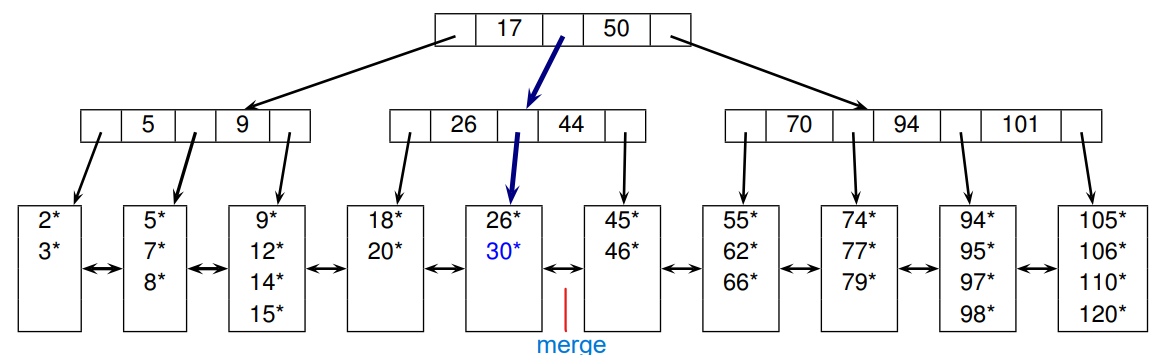
\includegraphics[width=7cm, height=2cm]{merge_nodes.png}
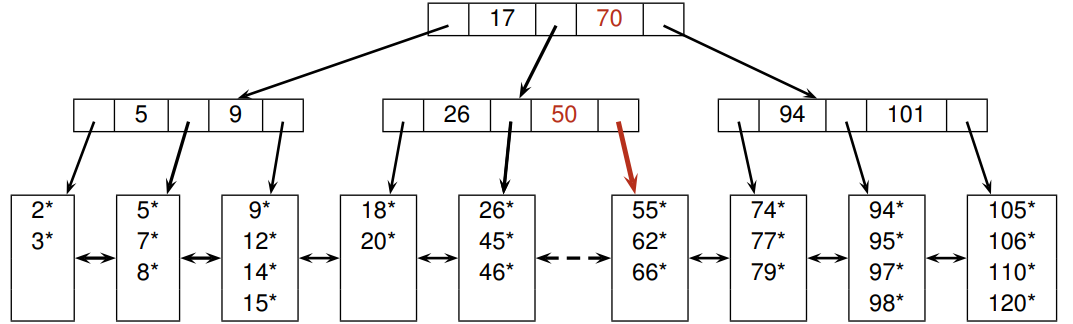
\includegraphics[width=7cm, height=2cm]{merge_parent.png}

\textbf{B+ Tree - Bulk Loading}
\begin{itemize}
  \item Initiazing a B+ tree by insertion is expensive (need to traverse tree n times)
  \item 1. Sort all data entries by search key
  \item 2. Initialise B+ tree with an empty root page
  \item 3. Load data entries into leaf pages 
  \item 4. In asc order, insert the index entry of each leaf page into the rightmost parent node
\end{itemize}


\textbf{Hash Based Index}
\begin{itemize}
  \item Does not support range search, only equality queries
\end{itemize}

\textbf{Static Hashing}
\begin{itemize}
  \item N buckets, each bucket has 1 primary page and $\geq$ 0 overflow pages
  \item To maintain performance, we need to routinely construct bigger hash tables and redistribute data entries
\end{itemize}

\textbf{Dynamic Hashing - Extendible Hashing}
\begin{itemize}
  \item No overflow pages! A bucket can be thought of as a page
  \item At most 2 Disk I/Os for equality search (at most 1 if directory and bucket fits in memory)
  \item Instead of maintaining data entries, we maintain pointers to data entries in buckets
  \item Instead of maintaining buckets, maintain a directory of pointers to buckets
  \item The directory has $2^d$ buckets, where d is the global depth --> large overhead if hashing is uniform
  \item Each director entry diffets by a unique d-bit adddress
  \item Two directories are corresponding iff their addresses differ only in the dth bit
  \item All entries with the same local depth (l) have the same last l bits in h(k)
\end{itemize}

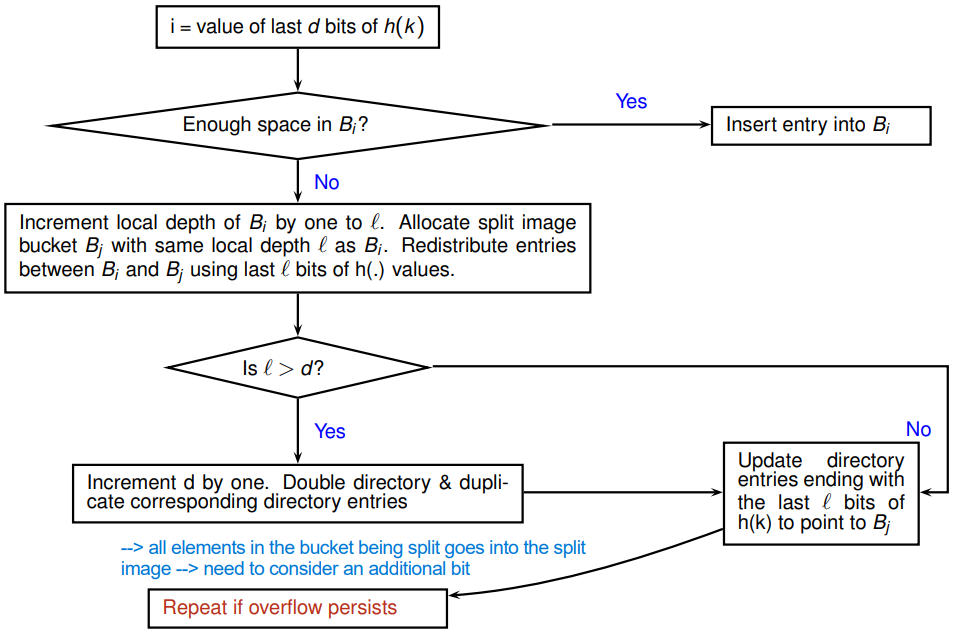
\includegraphics[width=7cm, height=4cm]{extendible_hash.png}
\textbf{Extendible Hashing - Split, Double}
\begin{itemize}
  \item Split and doubling is checked every time a bucket is full 
  \item Doubling only happens if local depth = global depth
  \item The split image has the same depth as the split bucket
  \item Other than the split image of the split bucket, split image of other buckets points to the same corresponding bucket
  \item Each bucket is pointed by $2^(d-l)$ directories
\end{itemize}

\textbf{Extendible Hashing - Deletion}
\begin{itemize}
  \item $B_i$ is deallocated
  \item l decrement by 1
  \item Directory Entries that point to $B_i$ points to its corresponding bucket
\end{itemize}

\textbf{Dynamic Hashing - Linear Hashing}
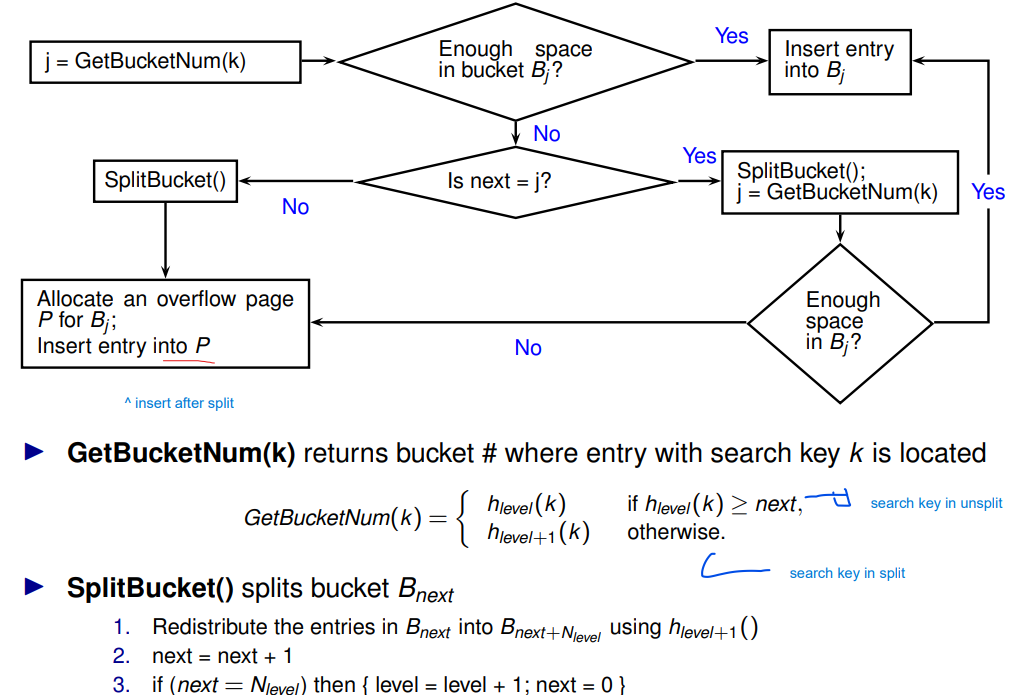
\includegraphics[width=7cm, height=4cm]{linear_hash.png}  
\begin{itemize}
  \item One I/O for equality search (more per number of overflow pages in bucket)
  \item Performs worse than extendible hashing if distribution is skewed
  \item Does not require a directory
  \item Higher average space utilisation, but longer overflow chains
  \item Has a family of hash functions, with each having a range twice of its predecessor
  \item $N_0$: initial number of buckets
  \item $N_i = 2^i N_0$: number of buckets at start of round i
  \item $next$: the next bucket to be split, this is incremented every time split happnes
  \item $h_i=h(k) mod N_{i}$: hash function for round i, if the bucket $\leq$ next (already split)
  \item $h_{i+1}=h(k) mod N_{i+1}$: hash function for round i+1, if the bucket $>$ next
  \item Split Citeria: By default, split when a bucket overflows
\end{itemize}

\textbf{Linear Hashing - Deletion}
\begin{itemize}
  \item Essentially the inverse of insertion
  \item If the last bucket is empty --> delete it and decrement $next$ by 1
  \item If $next$ is 0, set it to $M/2 - 1$, and we can decrement level by 1 (half of buckets have been deleted if $next$ is 0)
  \item Merging with corresponding bucket is optional
\end{itemize}

\section{L4: Query Evaluation - Sort, Select}
\textbf{Sorting - External Merge Sort}
\newline
Projection, join, bulk loading etc all require sorting

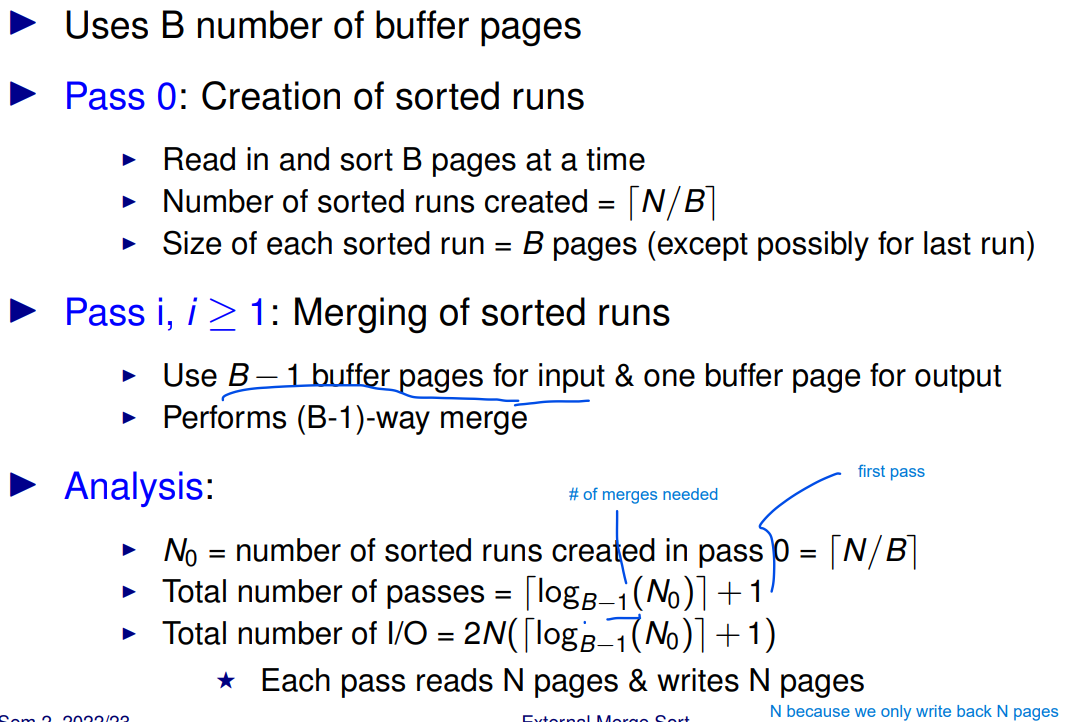
\includegraphics[width=7cm, height=4cm]{ext_sort.png}

\textbf{External Merge Sort - Bocked I/O}
\begin{itemize}
  \item Read and write in blocks of \textbf{b} buffer pages (replace b with 1 for unoptimised)
  \item $\floor{\frac{B-b}{b}}$ blocks for input, 1 block for output
  \item Can merge at most $\floor{\frac{B-b}{b}}$ sorted runs in each merge pass
  \item $F=\floor{\frac{B}{b}} - 1$ runs can be merged at each pass
  \item Num passes = $\log_{F} N_0$
\end{itemize}

\textbf{B+ tree sort}
\begin{itemize}
  \item B+ Tree is sorted by key
  \item Format 1 (clustered): Sequential Scan 
  \item Format 2/3:Retrieve data using RID for each data entry 
  \item Unclustered implies more I/Os
\end{itemize}

\textbf{Access Path} refers to the different ways to retrieve tuples from a relation. It is either a \textcolor{red}{file scan} or a \textcolor{green}{index plus matching selection condition}. The more \textbf{selective} the access paths, the fewer pages are read from the disk.
\begin{itemize}
  \item Table scan: scan all data pages 
  \item Index scan: scan all index pages 
  \item Table intersection: combine results from multiple index scans (union, intersec). Find RIDs of each predicate and get the intersection
\end{itemize}

\textbf{Query: Selection}
\textbf{Covering Index}
\begin{itemize}
  \item I is a covering index for query Q if I contains all attributes of Q
  \item No RID lookup is needed
  \item Index-only plan
  \item If data is unclustered, unsorted, no index -> best way is to collect all entries and sort by RID before doing I/O 
\end{itemize}

\textbf{CNF Predicate}
\begin{itemize}
  \item Find RIDs of each predicate and get the intersection
  \item Conjuncts are in the form (R.A op c V R.a op R.b) 
  \item CNF are conjuncts (or terms) connected by $\land$ 
\end{itemize}

\textbf{Matching Predicates - B+ Tree}
\begin{itemize}
  \item Non-disjunctive CNF (no $\lor$)
  \item At most one non-equality comparison operator which must be on the \textbf{last attribute in the CNF}
  \item $(k_1=c_1) \land (k_2=c_2) \land ...k_i op c_i | I=(k_1, k_2...k_n)$ 
  \item The order of k matters, and there cannot be missing $K_i$ in the middle of the CNF
  \item Having inequality operator before equality operator makes the query to be less selective 
\end{itemize}

\textbf{Matching Predicates - Hasing}
\begin{itemize}
  \item No inequality operators $(k_1=c_1) \land ... k_i =c_n | I=(k_1, k_2...k_n)$
  \item Unlike B+ tree, \textbf{all predicates must match}
\end{itemize}

I=(age, weight, height), p=($age \geq 20 \land age \geq 18 weight=50 \land height=150 \land level=3$) \newline
\textbf{Primary Conjuncts} : The subset of conjuncts in p that I matches \newline
Primary Conjuncts: $age \geq 20 \land age \geq 18$ \newline
\textbf{Covered Conjuncts} : The subset of conjuncts in p that I covers (conjuncts that appear in I). Primary conjunct $\subseteq$ covered conjunct \newline
Covered Conjuncts: $age \geq 20 \land age \geq 18 \land height=150$ \newline

\textbf{Cost Notation}  \newline
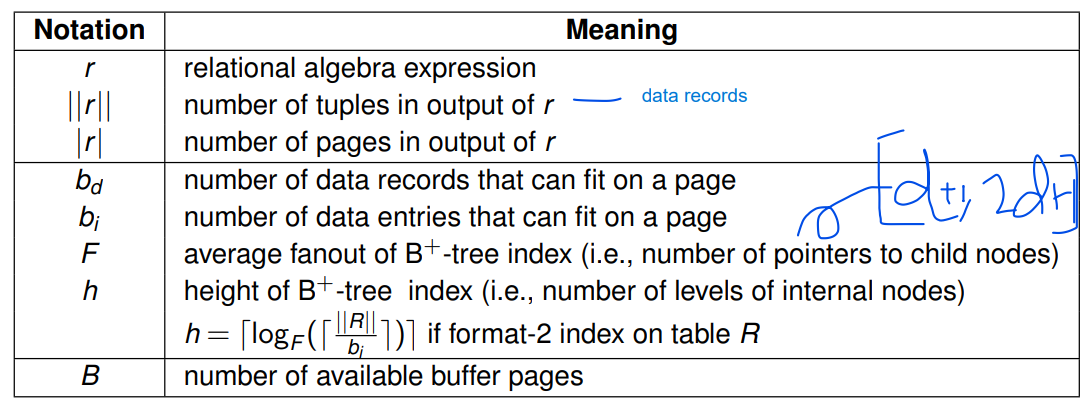
\includegraphics[width=5cm, height=3cm]{notation.png}

\textbf{Cost of B+-tree index evaluation of p} \newline
Let p'=primary conjuncts of p | $p_c$=covered conjuncts of p \newline
\begin{itemize}
  \item[1.] Navigate internal nodes to locate the first leaf page
  $$
  Cost_{internal} = \left\{
    \begin{array}{ll}
        \ceil{log_F(\ceil{\frac{||R||}{b_d}})} | Format 1 \\
        \ceil{log_F(\ceil{\frac{||R||}{b_i}})} | Otherwise
    \end{array}
\right.
  $$ \newline
  \item[1.1] This is traversing the height of B+ tree
  \item[2.] Scan leaf pages to access all qualifying data entries
  $$
  Cost_{leaf} = \left\{
    \begin{array}{ll}
        \ceil{\ceil{\frac{||\sigma_{p'}(R)||}{b_d}}} | Format 1 \\
        \ceil{\ceil{\frac{||\sigma_{p'}(R)||}{b_i}}} | Otherwise
    \end{array}
\right.
  $$ \newline
  \item[2.1] This is the cost of reading qualifying conjuncts
  \item[2.2] Using $p_c$ would be wrong since covering conjuncts may be non-matching which results in more reads from the leaves 
  \item[3] Retrieve qualified data records using RID lookups. 0 if I is covering OR format 1 index. $||\sigma_{p_c}(R)||$ otherwise
  \item[] 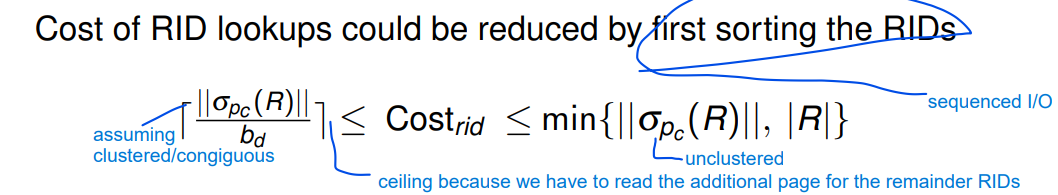
\includegraphics[width=5cm, height=1.3cm]{optimisation.png}
\end{itemize}

\textbf{Cost of Hash index evaluation of p}
\begin{itemize}
  \item Format 1: cost to retrieve \textbf{data entries} is at least$\ceil{\frac{||\sigma_{p'}(R)||}{b_d}}$
  \item Format 2: cost to retrieve \textbf{data entries} is at least $\ceil{\frac{||\sigma_{p'}(R)||}{b_i}}$
  \item Format 2: Cost to retrieve \textbf{data records} is 0 if it is a covering index (all information in data entry) OR $||\sigma_{p'}(R)||$ otherwise
\end{itemize}

\end{multicols}
\end{document}